\documentclass{deliverablereport}

\deliverable{hpc}{GAP-HPC-report}
\deliverydate{XX/YY/201Z}
\duedate{31/08/2019 (M48)}
\author{Author names}

\renewcommand{\comment}[1]{\TODO{Comment: #1}}
\begin{document}
\TODO{Author names}
\maketitle
% This will be the abstract, fetched from the github description
\githubissuedescription

% write the report here

% Original list of sections and subsections created from
% https://github.com/OpenDreamKit/OpenDreamKit/issues/113

\TODO{Write some preamble. Describe the structure of this report.}

\section{Developments in the core\GAP system}\label{core-gap}

This Section highlights some of the most important and relevant
changes to the core \GAP system incorporated in the new \GAP releases
published during the project. Other important developments are
included in \GAP packages and described in later sections.  More
detailed descriptions of each major and minor \GAP release, with links
to the corresponding source code changes on GitHub, are contained in
the ``GAP - Changes from Earlier Versions'' document, which is
redistributed with \GAP and also available on the \GAP website at
\url{https://www.gap-system.org/Manuals/doc/changes/chap0.html} and
included as an appendix to this report. This
work includes contributions from our external collaborators, whose
authorship can be seen from the version control history.

\subsection{\GAP 4.8 (February 2016)}\label{gap-4.8}

\GAP 4.8 was the first major release of \GAP published
after the start of the OpenDreamKit project.
As a preparation for the future developments to support multithreading, 
some language extensions from the HPC-\GAP project were backported to the 
\GAP library to help to unify the codebase of both \GAP 4 and HPC-\GAP. 

In addition, it also provided support for much enhanced
profiling. Previously \GAP\ allowed tracking of the CPU spent
executing each function, but the new features in
the core system reduced the granularity of this to individual lines of
\GAP code. Related developments also made it easier to track time
spent on individual lines of C code in the \GAP kernel. A related
feature makes it easy to measure ``test coverage'' -- the proportion
of the system that has actually been executed by a given set of
tests. The {\sf Profiling} package by
Christopher Jefferson (St Andrews) provided excellent tools for transforming these profiles
into various human-readable forms. These features 
supported later  work on enhancing both the performance and the
reliability of \GAP, through easier identification of hot-spots and
easier measurement of test quality.

This release also included some language extensions which would allow users to write
more efficient and readable code:
\begin{itemize}
  \item support for \emph{partially
  variadic functions} similar to those allowed in Python, allowing
function expressions like
\verb|function( a, b, c, x... ) ... end;|
which requires at least three arguments \verb|a|, \verb|b| and
\verb|c| and assigns
\item more flexible list indexing, allowing users to install methods
  for multiple indexing   (\verb|m[i,j]| instead of \verb|m[i][j]| for arrays) and more varied
  indexes (such as \verb|l[-1]| for a doubly-infinite virtual list. As
  well as being more flexible, this was a step towards supporting more
  efficient array implementations  in which ``row objects'' (like
  \verb|m[i]| in \verb|m[i][j]|) might not exist.
\end{itemize}

\GAP 4.8 had seven public releases between February 2016 and August 2017, and
was replaced by \GAP 4.9.

\subsection{\GAP 4.9 (May 2018)}\label{gap-4.9}

\GAP 4.9 continued the restructuring and modernising of the core \GAP
system. Aiming at the greater reliability, flexibility and performance
which would needed for \GAP to take full advantage of the \ODK ecosystem.
For example, we removed our old home-grown large integer arithmetic
implementation, and instead always 
use the state of the art external library \href{???}{GMP}. This
continues our cautious move to take more advantage of existing free
software libraries in the core system. We do this cautiously, based on
our experience,  so that we can maintain the reliability and
portability of \GAP on which our users depend.

Also for portability reasons, this release incorporated a  completely
reimplemented build system for \GAP, using more modern tools and
complying with modern expectatiuons. This resolved many issues with the old
system, and made it easier to maintain and extend. Technical details
of the new build system are described in {\tt README.buildsys.md} from
the \GAP source code. 

This also enabled us to merge the experimental code to support safe multithreaded programming in \GAP, 
dubbed HPC-\GAP, into the mainstream \GAP system as a compile-time option (for details, see
Subsection~\ref{hpc-gap}).

This release also incorporated many smaller performance improvements. For example,
\GAP now supports named constants, whose value cannot change 
at runtime. While maintaining readability through naming, uses of
these constants can be optimised as a function is parsed, so that they
are as fast as using explicit values. Another notable improvement was
to the widely used  sorting functions which have been improved using
recently published algorithms and made more maintainable by
restructuring the implementation.

Debugging  tools were improved: in many cases \GAP now outputs the
source filename  and location from which relevant code was originally
read as well as simply printing the lines of code or names of functions.

Further enhancements to the profiling system based on experience with
\GAP 4.8 were also included, as were additional changes improving \GAP
usability by allowing more
efficient and/or readable code,
\begin{itemize}
  \item a concise syntax for short
functions with any number of arguments such as \verb|{a,b} -> a+b| replacing \verb|function(a,b) return a+b; end|. 

\item use of function literals in expressions such \verb|y := f().x;| 
replacing \verb|y := f();; y := y.x;|).
\end{itemize}

\GAP 4.9 had three public releases between May and September 2019, and
was replaced by \GAP 4.10.

\subsection{\GAP 4.10 (November 2018)}\label{gap-4.10}

The release of \GAP 4.9 with the new build system allowed a
further restructuring of the core \GAP system to continue, and allowed
us to finalise a number of other ongoing changes, 
 resulting in the 
next major release just a few months later. \GAP 4.10 is current version
of \GAP, with the latest release being \GAP 4.10.2, published in June
2019 and \GAP 4.11 expected in September 2019.

The most important new feature in \GAP 4.10 was \texttt{libGAP} an
option to compile \GAP as a C library instead of a stand-alone
executable. This is discussed more in section \ref{libgap} below.

\GAP 4.10 also provides experimental support for using alternative
memory management systems, notably the \href{??}{Julia} garbage
collector and the \href{???}{Boehm garbage collector} in place of
the GASMAN system which was developed for \GAP 4 in the 1990s.
These garbage collectors are thread-safe (important for \HPCGAP) the
links to Julia are
motivated by a desire to allow tight integration with \GAP and Julia 
in the future, led by  the DFG-funded OSCAR project.
% TODO: proper reference to OSCAR

The work on improving debugging and profiling in \GAP was
continued. Profiling now covers memory usage as well as CPU time, and
additional checking options (internal and using external tools such as
\href{???}{valgrind}) help to detect misuse of memory in the kernel.

Using the improved debugging and profiling facilities we were able to detect many
performance bottlenecks and confirm that new code was both correct and
genuinely improved performance.
For example, the method selection code was rewritten from \GAP to C;
Speed ups were achieved for many integer arithmetic functions such as
\verb|GcdInt|, \verb|LcmInt|, \verb|PValuation|, 
\verb|RootInt|, \verb|SmallestRootInt|, \verb|IsPrimePowerInt|
and the computation of modular inverses of integers.

For example (this could be converted into a table):

{\small
\begin{verbatim}
gap> q:=1/3^60;;n:=2^59;; for i in [1..2000000] do x:= q mod n; od; time;
2364
gap> q:=1/3^60;;n:=2^60;; for i in [1..2000000] do x:= q mod n; od; time;
2821
gap> q:=1/2^6000;;n:=3^6000;; for i in [1..6000] do x:= (q mod n); od; time;
19358
\end{verbatim}
}

After:

{\small
\begin{verbatim}
gap> q:=1/3^60;;n:=2^59;; for i in [1..2000000] do x:= q mod n; od; time;
1219
gap> q:=1/3^60;;n:=2^60;; for i in [1..2000000] do x:= q mod n; od; time;
1292
gap> q:=1/2^6000;;n:=3^6000;; for i in [1..6000] do x:= (q mod n); od; time;
692
\end{verbatim}
}

Also, \verb|InverseMatMod| with integer modulus has been improved:% #2426

TODO: convert into a table

{\small
\begin{verbatim}
gap> m2:=RandomUnimodularMat(100);;
gap> for i in [1..100] do x:=InverseMatMod(m2,2); od; time;
277
gap> for i in [1..100] do x:=InverseMatMod(m2,251); od; time;
1564
gap> for i in [1..100] do x:=InverseMatMod(m2,65537); od; time;
Error, reached the pre-set memory limit
\end{verbatim}
}

After:

{\small
\begin{verbatim}
gap> m2:=RandomUnimodularMat(100);;
gap> for i in [1..100] do x:=InverseMatMod(m2,2); od; time;
273
gap> for i in [1..100] do x:=InverseMatMod(m2,251); od; time;
1249
gap> for i in [1..100] do x:=InverseMatMod(m2,65537); od; time;
1226
\end{verbatim}

}

The same improved profiling tools allowed us to identify other
``hidden'' bottlenecks in \GAP code. For instance \GAP has a
sophisticated system of inference that can trigger 
so-called ``immediate methods'': quick attempts to deduce additional
consequnces from information that becomes known about an object.
In general, these are very effective, and the deduced information can
lead the system to chose better methods for subsequent
calculations. As an example arises when a group learns its order, we
can check if that order is finite and odd, and if so, thanks to the celebrated
Feit-Thomson theorem, conclude that the group is solvable. Once that
is known, much more efficient methods can be applied for many
subsequent calculations.

While this is a very powerful feature in most situations, there can be
rare examples where a large number of short-lived objects are created,
and the immediate methods use a great deal of time deducing knowledge
that will never be used. The profiling developments made this 
easily visible for the first time, and some small adjustments to the
immediate methods produced up to a six-fold speed up in fundamental
operations such as computing isomorphism groups. For instance the
run-time for the code fragment below on a test system dropped from 130
seconds to 22.


{\small
\begin{verbatim}
G:=PcGroupCode( 
  741231213963541373679312045151639276850536621925972119311,
  11664);;
IsomorphismGroups(G,PcGroupCode(CodePcGroup(G),Size(G)))<>fail;
\end{verbatim}
}


\subsection{\GAP 4.11 (anticipated ???? 2019)}\label{gap-4.11}

% Since they are released on GitHub, I see no reason not to also
% highlight changes which are merged and definitely coming out in
% 4.11, if they are relevant SL

At the time of preparation of this report the next major release \GAP
4.11 is approaching completion. Almost all of the features to be
included in it (including all the ones highlighted here) are already
publicly  available on GitHub to developers or anyone else interested.

This will feature the first release of the ``syntaxtree'' reflection
API for \GAP, allowing \GAP to access and modify the internals of \GAP
functions, opening up a range of possibilities for optmisation, automatic
parallelisation, and more effective compilation into C. This is
discussed in more detail in section \ref{syntaxtree} below. 

Additional relevant features are continued improvements to debugging and
profiling facilities \TODO{maybe some examples} extensions to the
\texttt{libGAP} API to allow programs using the system in this way
more convenient access to \GAP objects; and a range of performance
enhancements.

\TODO{is there more?}

% What about making pages for relevant releases in
% https://www.gap-system.org/Manuals/doc/changes/manual.pdf 
% (or print HTML version of the manual into PDF)
% an electronic appendix to the deliverable?
%
% Yes -- let's do that. Add them as appendices.
%
% Indeed, as the ODK README.md says:
%
%  The report shall be self-contained. Indeed, the
%  deliverable will be evaluated based upon its version submitted on
%  the EU portal without retrieving other resources. Links have no
%  legal value, since there is no guarantee that the referenced
%  material will remain unchanged. One may typically want to add
%  relevant material as appendix (e.g. snapshots of software
%  documentation, websites, or other relevant documents); see e.g.
%  [WP5/D5.1/report.tex](WP5/D5.1/report.tex) or
%  [WP2/D2.1/report.tex](WP2/D2.1/report.tex).

\TODO{Can we assemble some statistics to show the general progress of
  work on \GAP performance and robustness over the project -- number
  of tests, maybe run the 4.8 or 4.7 testinstall in 4.7 and 4.11 and
  compare performance?}


\subsection{lib\GAP: allowing 3rd party code to link \GAP as a library}\label{libgap}

The initial connection between \Sage and \GAP was developed around
2006, and relied on running a full \GAP process with which \Sage
communicated through pipes, creating \GAP input as text and parsing
the text output by \GAP. This enabled an initial connection, but
introduced considerable overhead coverting objects to and from text
representations and passing them between processes.

A better solution is to provide a C API enabling \GAP to be integrated
into the \Sage process, and allowing a \GAP session to be started,
objects created, functions called and results retrieved via C function
calls. This is, however, not a mode of operation for which \GAP was
ever designed, and implementing it in a robust and flexible way
required considerable adaptations to the system, for instance to make
sure it never tried to access the terminal. Based on an iniital
version developed within the \Sage team, a fully general-purpose and
flexible version was released in  \GAP 4.10.0 (November 2018).

Subsequent releases have improved and will continue to improve the
robustness of lib\GAP, and to extend its API with new functionality (See Chapter 2 
``Changes between \GAP 4.9 and \GAP 4.10'' of the 
``\GAP - Changes from Earlier Versions'' manual for the detailed
descriptions). This has allowed \Sage to drop its custom 
modifications to \GAP and use an official, documented and regularly 
tested \GAP interface instead, starting from SageMath 8.6 (January
2019).

% See SageTrac ticket 22626 made that happen; it was merged in 
% SageMath 8.6.beta0, so SageMath 8.6 had it but not SageMath 8.5.

\subsection{Reflection}\label{syntaxtree}
\TODO{write this}

\section{High-performance computing with \GAP}\label{hpc}

\subsection{HPC-\GAP: multithreaded programming in \GAP}\label{hpc-gap}

\GAP 4.9.1 (May 2018) for the first time included experimental code to 
support safe multithreaded programming in \GAP, dubbed \HPCGAP. This
has been in development for some time, and the \HPCGAP and \GAP
codebases had diverged. In this release we unified the codebases,
making thread support a compile-time option instead of completely
different programme. This was an essential step to support further development of 
HPC-\GAP, and ensure that new developments in \GAP could be quickly
incorporated.
It also provided users an opportunity to start to experiment 
with \HPCGAP, for which documentation is also provided.

\HPCGAP supports two models of parallel programming in \GAP, which can
be combined: threads and tasks. Threads operate as in most languages,
teh basic primitive is to start execution of a \GAP function in a new
thread, while the calling thread returns immediately. Threads can
interact through global data or by returning results when they exit. Tasks are
similar, but they are submitted to a shared job queue and executed by
one of a fixed-size pool of worker threads. Typically the calling
process will start a number of threads and then wait for somne or all
of them to complete.  Supporting this requires considerable work on
the \GAP interpreter, but is otherwise straightforward.

The challenge
however is that the \GAP library makes very extensive use of shared
global data, which is frequently updated as new knowledge is
obtained. Ensuring that access and updates to this data from different
threads and tasks does not cause corruption or inconsistency was the
main challenge. The approach taken was to limit access, in most cases,
to data ``owned'' by the accessing thread; read-only data and
``public'' data stored in thread-safe data structures. This is
implemented by access checks in the kernel with the aim of ensuring
that most unsafe data access should result in error messages, rather
than inconsistent results. Experiments with this system have been
reported in a number of papers.

The main remaining challenge is to adapt the enormous legacy codebase
represented by \GAP's library and key packages to use these mechanisms
effectively, and to keep the underlying mechanisms working as the core
\GAP codebase evolves. Fusing the codebases, as was done in \GAP 4.10
was a critical step in this work, meaning, for instance, that all
changes to \GAP are tested in \HPCGAP automatically.


% Release announcement: https://www.gap-system.org/Manuals/doc/changes/chap3.html#X7F52B77B7DBACC17

% HPC-\GAP manual: https://www.gap-system.org/Manuals/doc/hpc/chap0.html

% What about making https://www.gap-system.org/Manuals/doc/hpc/manual.pdf 
% an electronic appendix to the deliverable?

\section{meataxe64: high-performance linear algebra over finite fields}\label{meataxe64}

A key kernel for many applications of \GAP is linear algebra over
a wide range of finite fields. This is used directly in working with
matrix groups and in computational representation theory, but also
arises indirectly in areas such as graph theory, finite solvable
groups and number theory. The \GAP kernel includes memory-efficient
representations of matrices over these fields, and implementations
based on the C-meataxe (the name ``meataxe'' is derived from the
abbreviation ``mtx'' for ``matrix'' and the fact that a key operation
in computational representation theory is to ``chop'' a module into
its irreducible components) from the late 1980s.

Working with external collaborators (primarily Richard Parker),
we have contributed to the design and development (and continue to extend) of a new C and
assembler library, called ``meataxe64'' which takes
advantage of new algorithmic ideas, and of powerful features of new
CPUs to deliver a quantum leap in performance. We have implemented a
\GAP interface to it (the ``meataxe64 \GAP package'') currently in
beta-test, and are in the
process of revising higher levels of the software stack to make best
use of it.

% TODO get some timings once I have a power supply.
% last time I tried, Monster-sized (196882 over GF(2)) multiply took
% 8 minutes on my laptop using 12 threads and 3 minutes on Ladybank
% using 64!) Should do Gaussian and try and get some timings
% comparable to GAP kernel timings.

% TODO: make a release at https://github.com/gap-packages/meataxe64/
% and publish it at https://gap-packages.github.io/meataxe64/
%  What does this need done? -- SL


\section{Regression testing, Package management and Release management}\label{gap-infra}

In this section we will describe mostly the technical aspects of
ensuring that all developments are becoming available to users.
The social aspects such as community building, user training
and technical support will be described in Section~\ref{gap-support}.

\subsection{Regression testing}\label{testing}

\emph{Regression testing} is a software engineering technique which uses
a set of tests to check (preferably in some automated way)
that new changes do not break the functionality that used to 
work previously. If a change breaks the test, that is called 
a \emph{regression}. In \GAP, regressions may occur, for example,
when a change causes an incorrect result, or a crash, or an error
message; in addition, there may be \emph{performance regressions}
and \emph{memory regressions}.

GAP regression testing uses \emph{integration tests} - these are
the tests when different parts of the \GAP functionality are 
exercised in the same \GAP session (opposite to \emph{unit tests}
which exercise each logical unit of the code separately, but do
not necessarily test interactions between them).\comment{Is this true?
  -- all tests are with an integrated system, but increasingly, each
  test covers narrow functionality}
The \GAP test
suite consists of a number \comment{what number?} of test files in the
{\tt tst} directory, \comment{can we also give some measure of total size} 
as well as of the tests that check the correctness of manual examples
\comment{again, numbers?}.
% and some further code in the {\tt benchmarks} directory. 

GAP is also redistributed with a number of extensions, called \GAP packages
(145 in the latest release \GAP 4.10.2). These packages may, for example,
extend mathematical functionality of the system by implementing new algorithms;
provide collections of mathematical data; or provide enhanced tools for 
package developers. Packages can be published independently of the core \GAP
system and have a separate authorship. Package authors are recommended to 
use a similar approach to testing and to provide their own regression tests.
For packages redistributed with \GAP, our automatic package update system
checks regularly for new versions on the authors web pages, retrieves them, and then uses them in a
number of checks to ensure that new package releases are compatible with
each other and do not break the functionality of the core \GAP system. The
same process also helps us to check that changes in the core \GAP system
do not break the functionality of the packages redistributed with \GAP
%% (provided those packages have standard tests that allow us to do that
%% automatically)
. This system has dramatically simplified the process of making a \GAP
release or update, for which we want a mutually compatible set of
package versions, also compatible with the new core system. This used
to require extensive negotiation with package authors, and sometimes
took months, even though the number of packages was much smaller. Now
developers have continuous visibility of the functionality and
compatibility of released and upcoming versions of packages and of the
core system, and releases are much faster.

\comment{Tenses in the next para are confused. This is all past, I
  think, and is also maybe a bit too much about stuff that happened
  before the project, before we get to anything new. Can we start by
  saying what new developments we are claiming, and then go back and
  explain what didn't work before?}
  
  \comment{Also maybe a subheading of some kind here}
\GAP has used regression tests in one or another form since the
release of version 3 in the 1980s. For much of this time, they were
run by developers manually, and a part of the
release preparation was sending an email to the \GAP developers mailing
list asking for help with running a set of tests on developers' 
computers. Since 2009, the \GAP team in St Andrews started to use the Jenkins
(\url{https://jenkins.io/}) automation sysetem to regularly run the 
GAP testsuite, and eventually established a set of nightly and weekly
running Jenkins jobs to run tests for the current \GAP development
version; check for package updates; prepare and test release candidates,
and other tasks. The system can keep and archive of test logs, and notify
developers when tests fail; however, the biggest limitations are that
it is not public and can be accessed only within St Andrews, and that 
it runs tests for changes that are \emph{already} in the development
version of \GAP, instead of checking them in advance. We understood
that one of the limiting factors (not only for the testing, but for
the \GAP development in general is that while \GAP is an open source 
software, it does not follow an open development model and does not
have a public source code repository. 


%See https://blogs.cs.st-andrews.ac.uk/alexk/2016/03/07/gap-on-github-one-year-on/
Of course, \GAP is not new  version control, and the former
CVS repository for \GAP 4 has revisions from 1996. In summer 2012 it
had been converted to Mercurial (thanks to Max Horn) after the release 
of \GAP 4.5, and then in February 2015 the Mercurial repository had 
been converted to Git (thanks to Chris Jefferson) and placed on GitHub
at \url{https://github.com/gap-system/gap}.

\comment{So the move to GitHub was just before the start of the
  project. So I guess our claim in this report is that we have
  consolidated \GAP development around GitHub and its tool ecosystem
  (maybe mention that we can break out onto GitLab if GitHub goes
  phut). I'd start with that.}
  
Hosting GAP repository on GitHub and eventual establishing of a number
of other repositories under the gap-system and gap-packages 
organisations (\url{https://github.com/gap-system} and 
\url{https://github.com/gap-packages}), and encouraging package authors 
to follow the same practices (see \url{https://gap-packages.github.io/})
to find some further packages that are having public source code 
repositories elsewhere) allowed us to bring our regression testing
up to the next level.

We made use of \href{https://travis-ci.org/}{Travis CI} and
\ref{https://www.appveyor.com/}{AppVeyor} which are 
free (for open source projects) continuous integration platforms 
that can be used to build and test software projects hosted at GitHub.
\emph{Continuous Integration}, usually abbreviated as {\bf CI} is the process
automated building and testing for every performed or suggested changes to 
the source code repository. Using Travis and AppVeyor, one can test changes proposed
in a pull request \emph{before} they are merged into the main repository.
At the moment, we use Travis CI for tests on Linux and macOS, and 
AppVeyor for tests on Windows.

In addition to that, we started to use \href{https://codecov.io/}{Codecov}
platform to collect \emph{code coverage} reports for GAP to ensure that our
regression tests exercise GAP codebase at an acceptable level, and then
the changes which are submitted via pull request are actually being tested
by Travis CI. Making this results easily obtainable and publicly available
had a great effect on the community. Adding new tests to improve code coverage
is a useful task for new contributors to familiarise themselves with the
project setup. Making coverage reports available for each pull requests
stimulated their authors to ensure that their contributions have a good
quality and their suggested changes are actually being tested.

A crucial role in these developments was played by the enhanced
profiling facilities and the {\sf Profiling} package by Christopher
Jefferson (St Andrews), described in Subsection~\label{gap-4.8}. 
GAP~4.8 also introduced the {\tt TestDirectory} function to find
(recursively) all {\tt .tst} files from a given directory or a list of 
directories and run them using {\tt Test}. Having ability to test
changes more efficiently also allowed us to further improve all 
tools involved in testing, making their output more informative,
and allowing test integration into various automated workflows
by a better detection of the test outcomes.

Figure~\ref{fig:gap-core-tests} displays a part of the dashboard
available at \url{https://github.com/gap-system/gap-distribution/}.
The ``status'' buttons lead to the test reports on Travis CI, and
the ``code coverage'' buttons lead to the code coverage reports on
Codecov. The coverage is shown for the latest revision in the
corresponding branch (release branches {\tt stable-4.9} and {\tt stable-4.10},
and the master branch which is the prototype of the coming GAP~4.11 release).

\begin{figure}[!ht]
    \centering
    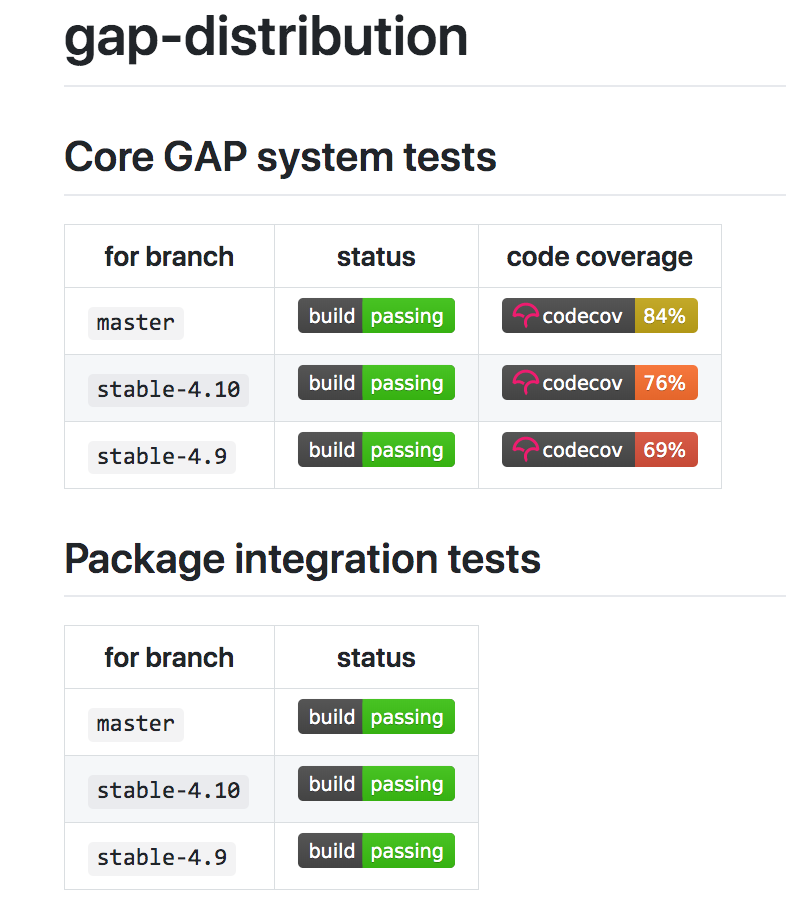
\includegraphics[width=5cm]{images/gap-core-tests}
    \caption{Dashboard with core GAP system and package integration tests}
    \label{fig:gap-core-tests}
\end{figure}

The top part of Figure~\ref{fig:gap-core-tests} shows core system GAP tests,
which are run for every change made to the repository. The bottom part shows
tests which are run once in 24 hours using a Docker container which is built
using a snapshot of the GAP development version on the moment of its creation
and a selection of GAP packages (including their updates, not yet redistributed
with GAP). Clicking on the ``status'' button will lead to the overview displayed
on Figure~\ref{fig:gap-docker-master-testsuite}, from where one could inspect
test logs for each of the configurations and see the diagnostics in case of a
test failure.

\begin{figure}[!ht]
    \centering
    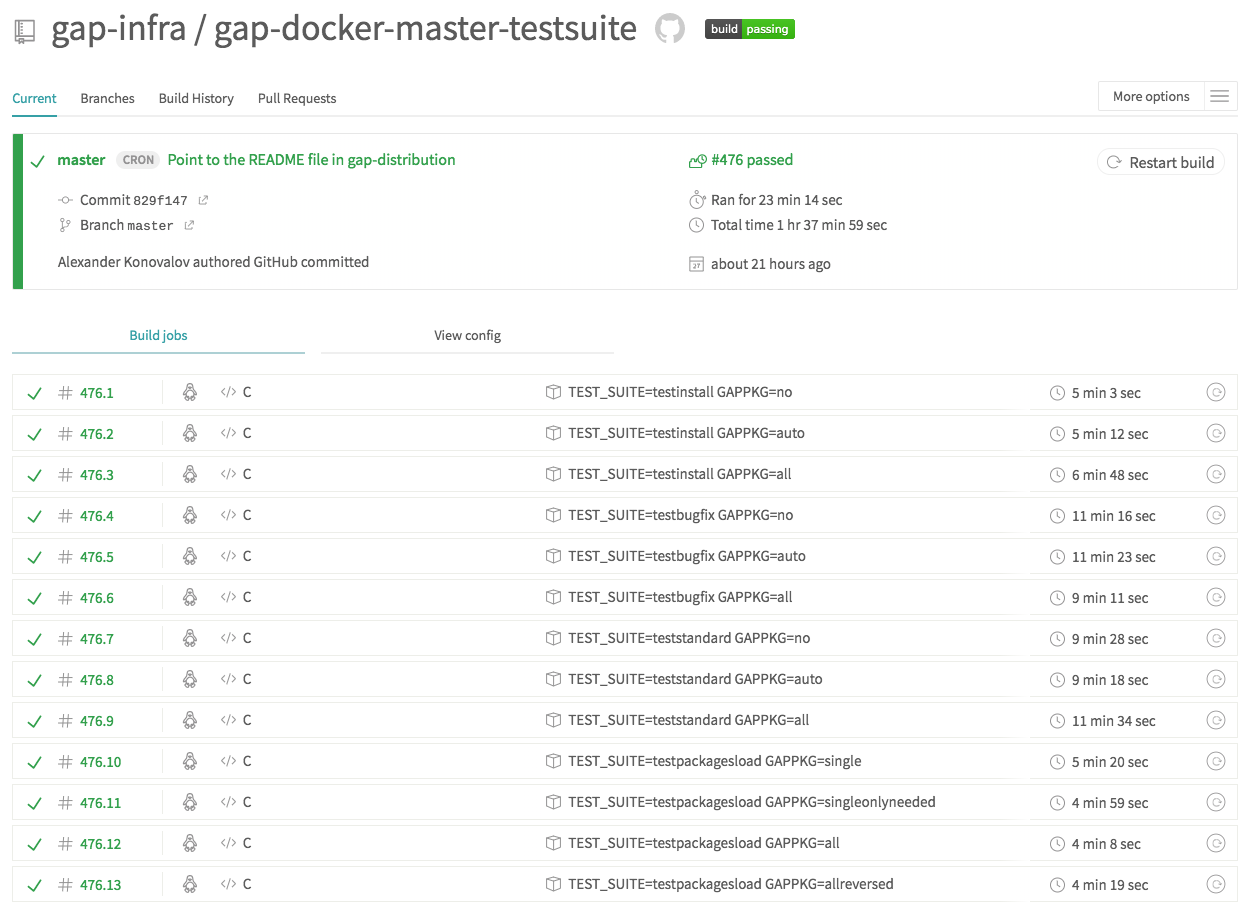
\includegraphics[width=\textwidth]{images/gap-docker-master-testsuite}
    \caption{GAP package integration tests on Travis CI}
    \label{fig:gap-docker-master-testsuite}
\end{figure}

The Docker container for the test displayed on Figure~\ref{fig:gap-docker-master-testsuite}
is one of a set of containers that we maintain for various purposes, from offering 
them as alternative distributions (see Subsection~\ref{distro}) or components for shareable
reproducible experiments (see Section~\ref{demos}), to ways to speed up regression tests running
container-based tests on Travis CI. These containers are publicly available on Docker Hub
(see Figure~\ref{fig:gap-docker}).
\comment{The Docker stuff might deserve to be its own section}

\begin{figure}[!ht]
    \centering
    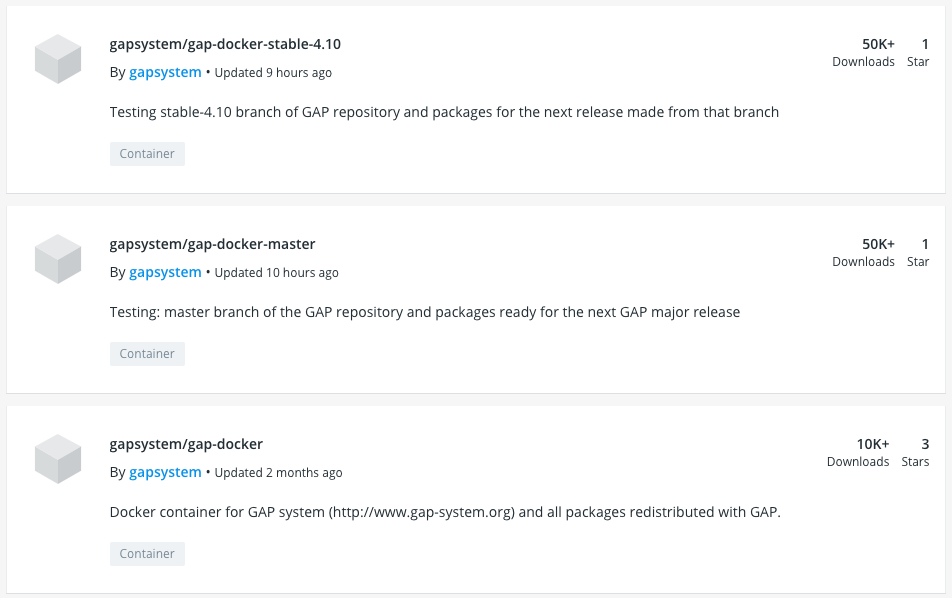
\includegraphics[width=12cm]{images/gap-docker}
    \caption{Selected GAP Docker containers on Docker Hub}
    \label{fig:gap-docker}
\end{figure}

At the same time, we continue to use Jenkins installation in St Andrews 
for daily and weekly tests, running package updates system, wrapping and
testing release candidates and other tasks. It is also very valuable since 
it does not impose time limits on output inactivity and the overall duration
of the job; second, it allows us to log in into the test workspace for
debugging; third, with the specific GAP setup for Windows we build it on a
machine with a Cygwin installation, and then install it on a clean Windows
machine to test there. 

\section{\GAP Packages}\label{packages}

Developments, described in the previous section, together with community
supporting activities described in Section~\ref{gap-support}, had substantial
impact on on the health of the package ecosystem. In the duration of the OpenDreamKit
project, we have observed the growth of the number of GAP packages and package 
authors, improvements in the quality of package testing, more frequent
package updates, and the development of a set of tools that appeared and helped to package authors. 

nd helped to package authors. 


Which tools we provide to support packages.

PackageMaker: (by Max Horn) https://github.com/gap-system/PackageMaker 

Example package: https://github.com/gap-packages/example 

ReleaseTools (by Max Horn): https://github.com/gap-system/ReleaseTools 

GitHubPagesFor\GAP (by Max Horn): https://github.com/gap-system/GitHubPagesFor\GAP 

Docker containers: https://hub.docker.com/r/gapsystem/ 

Standard setup for Travis CI and CodeCov (by Max Horn et al.)

AutoDoc

Add screenshots from Travis and CodeCov for packages



Figure~\ref{fig:gap-package-releases} shows how package releases became more frequent.
Now the oldest package is released in 2012, and the majority is 2018--2019. 
This means that packages are updated to make use of the recent \GAP developments,
they are responsive to reports about detected problems; hosting packages on GitHub
facilitates that; we can help by submitting PRs and publish releases for authors,
who prefer to overlook mathematical functionality and general development of the
package but do not want to dive into technicalities of release wrapping.

\begin{figure}[!ht]
    \centering
    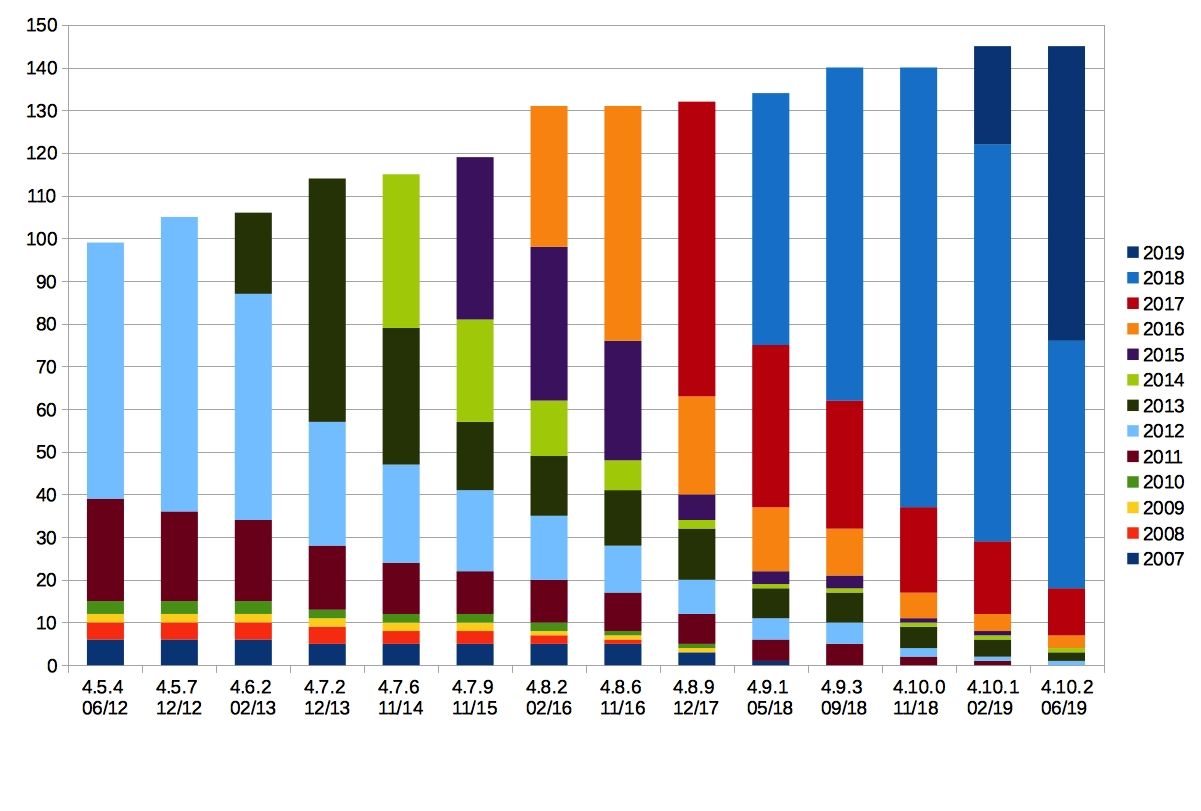
\includegraphics[width=\textwidth]{images/gap-package-releases}
    \caption{Number of \GAP packages and their release year}
    \label{fig:gap-package-releases}
\end{figure}

Figure~\ref{fig:gap-package-releases} shows that not only
package releases became more frequent, but also their quality
improved. We are able to tests more packages, and tests pass
for more packages. At the same time, community grows - it
shows the number of package authors.

\begin{figure}[!ht]
    \centering
    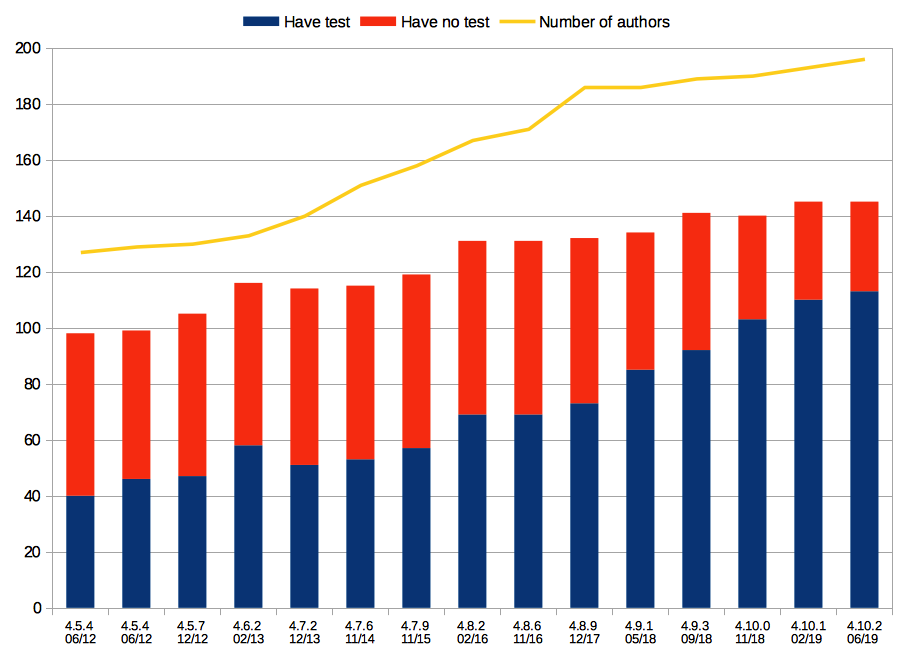
\includegraphics[width=\textwidth]{images/gap-package-tests}
    \caption{Number of \GAP packages, their authors, and packages with tests.}
    \label{fig:gap-package-tests}
\end{figure}

\subsection{\GAP package manager}\label{pkg-manager}

WHO: Michael

Describe \url{https://gap-packages.github.io/PackageManager/}

\subsection{Packaging \GAP distribution}\label{distro}

WHO: Alex

When we decide that there is a time for the next release
(minor or major; update releases were in the past but then abolished).
What are the standards for passing tests. 

How release wrapping is automated.
Which \GAP distributions we provide officially.

Figure~\ref{fig:gap-package-releases} shows how package releases became more frequent.

\begin{figure}[!ht]
    \centering
    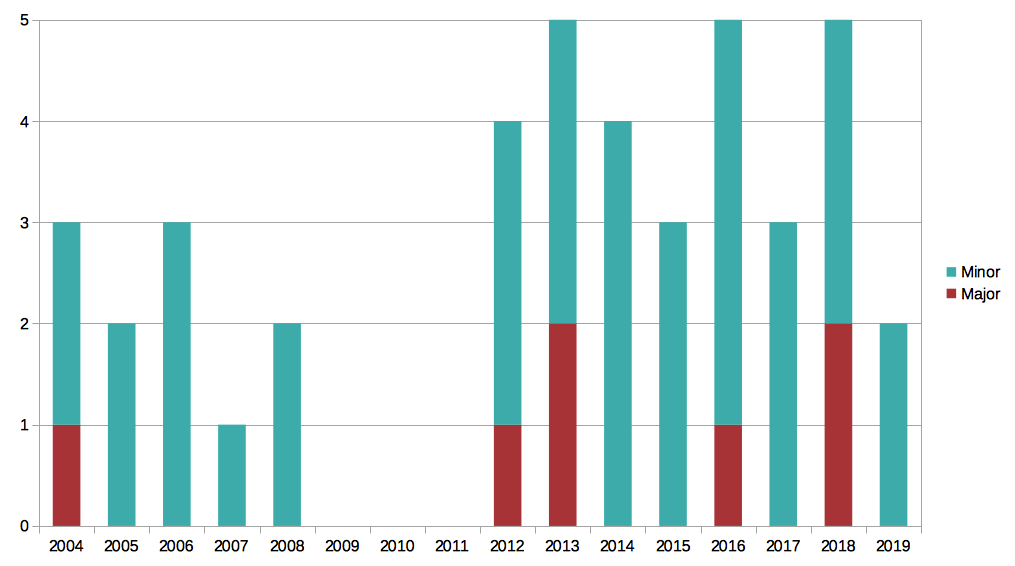
\includegraphics[width=\textwidth]{images/gap-releases}
    \caption{Number of major and minor \GAP releases per year since \GAP 4.4 release.}
    \label{fig:gap-releases}
\end{figure}

Main distributions
Regression testing
Windows distribution and installer migrated from Windows 7 to Windows 10
Alternative distributions: Docker, Homebrew, 
Opportunity to try \GAP online with Jupyter notebook running on Binder.
Improved testing
Code coverage, various sets of automated Travis builds
This is based on Docker containers for various branches.

\section{Jupyter interface to \GAP}

WHO: Alex, with help from and Michael

TODO: Refer to previous deliverables and describe how their outputs
evolved and any impacts they achieved

JupyterKernel has been reported in DX.Y. Since that, there were
several more releases of the kernel, associated with new \GAP
releases, improving its robustness. 

JupyterKernel lead to several follow-up developments, their
functionality will be described below: Francy, JupyterViz,
other work by Nathan Carter (also mention related work on
GroupExplorer).

Have used in in teaching and in explaining how to share 
reproducible experiments that use \GAP. Using Binder
allows to try \GAP in Jupyter online. Provide details
and consider including an appendix with an example 
demonstrating the setup.

\section{Community building, Technical support, User Training and Dissemination}\label{gap-support}

WHO: Alex

Describe all training events, Software Carpentry lesson, other workshops

\section{Interfaces, WP6}

WHO: Michael

Fix title of the section.

High-level interoperability

Persistent memoisation

\section{A collection of demonstrators}\label{demos}

For example:

Reproducible experiments with Jupyter

``full-stack semigroups''

persistent memoisation

databases

% TODO: Bibliography. Ensure that we are following software citation recommendations properly!
\end{document}


%%% Local Variables:
%%% mode: latex
%%% TeX-master: t
%%% End:

